\documentclass[logo,reportComp]{thesis}
\usepackage[cpp,pseudo]{mypackage}
\usepackage{forest}

\usetikzlibrary{automata,backgrounds,fit,shapes,positioning}

\tikzset{->, % makes the edges directed
>=stealth, % makes the arrow heads bold
node distance=2.5cm, % specifies the minimum distance between two nodes. Change if necessary.
every state/.style={thick, fill=gray!10}, % sets the properties for each 'state' node
}

\forestset{
sn edges/.style={for tree={edge={-}}}
}

\title{编译原理作业十}
\subtitle{}
\school{数据科学与计算机学院}
\author{陈鸿峥}
\classname{17大数据与人工智能}
\stunum{17341015}
\headercontext{编译原理作业}


\begin{document}

\maketitle

\begin{question}
考虑以下基本块:
\[\begin{aligned}
t_0 &= 5\\
t_1 &= 3 * t_0\\
t_2 &= R + r\\
t_3 &= t_1 * t_2\\
t_4 &= t_2\\
t_5 &= t_3 - t_4\\
t_6 &= t_1 * t_2\\
A   &= t_6 + t_5\\
B   &= A - r\\
t_7 &= t_1\\
B   &= t_7 + B
\end{aligned}\]
\begin{enumerate}
\item 构造这一基本块的DAG.
\item 假设只有$A$和$B$在基本块后面还要被引用,产生优化后的三地址代码.
\end{enumerate}
\end{question}
\begin{answer}
\begin{enumerate}
	\item 基本块的DAG如下图所示
	\begin{figure}[H]
	\centering
	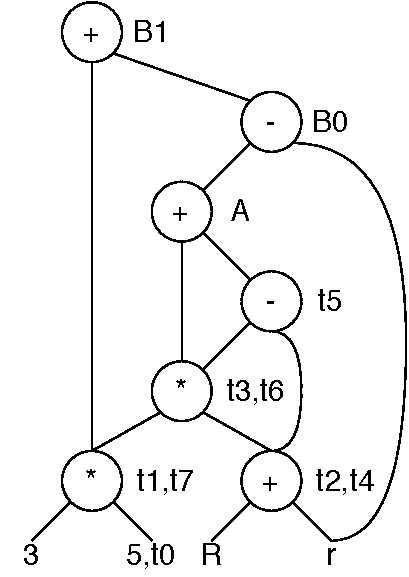
\includegraphics[width=0.4\linewidth]{fig/dag-1.pdf}
	\end{figure}
	\item 优化后的三地址代码如下
\[\begin{aligned}
t_1 &= 3 + 5\\
t_4 &= R + r\\
t_3 &= t_1 + t_4\\
t_5 &= t_3 - t_2\\
A &= t_3 - t_5\\
B &= A - r\\
B &= t_1 + B
\end{aligned}\]
\end{enumerate}
\end{answer}

\begin{question}
考虑下列代码片段:
\begin{enumerate}[label=(\arabic*)]
\item \verb'm := 0'
\item \verb'v := 0'
\item \verb'if v >= n goto (19)'
\item \verb'r := v'
\item \verb's := 0'
\item \verb'if r < n goto (9)'
\item \verb'v := v + 1'
\item \verb'goto (3)'
\item \verb's := v + r'
\item \verb'y := 0 * x'
\item \verb'z := v - y'
\item \verb'x := z + r'
\item \verb'r := m - x'
\item \verb'if s <= m goto (17)'
\item \verb'm := s'
\item \verb's := s + r'
\item \verb'r := r+1'
\item \verb'goto (6)'
\item \verb'return m'
\end{enumerate}
为这段代码划分基本块(Basic Block),并画出控制流图(Control Flow Graph).
在答案中你可以直接画出控制流图,但对图中的每个结点,请用$m\thicksim n$表示相应的基本块由第$m$至第$n$条语句组成.
\end{question}
\begin{answer}
如下图所示,共$9$个基本块,每个基本块包含的语句已在图中标出。
\begin{figure}[H]
\centering
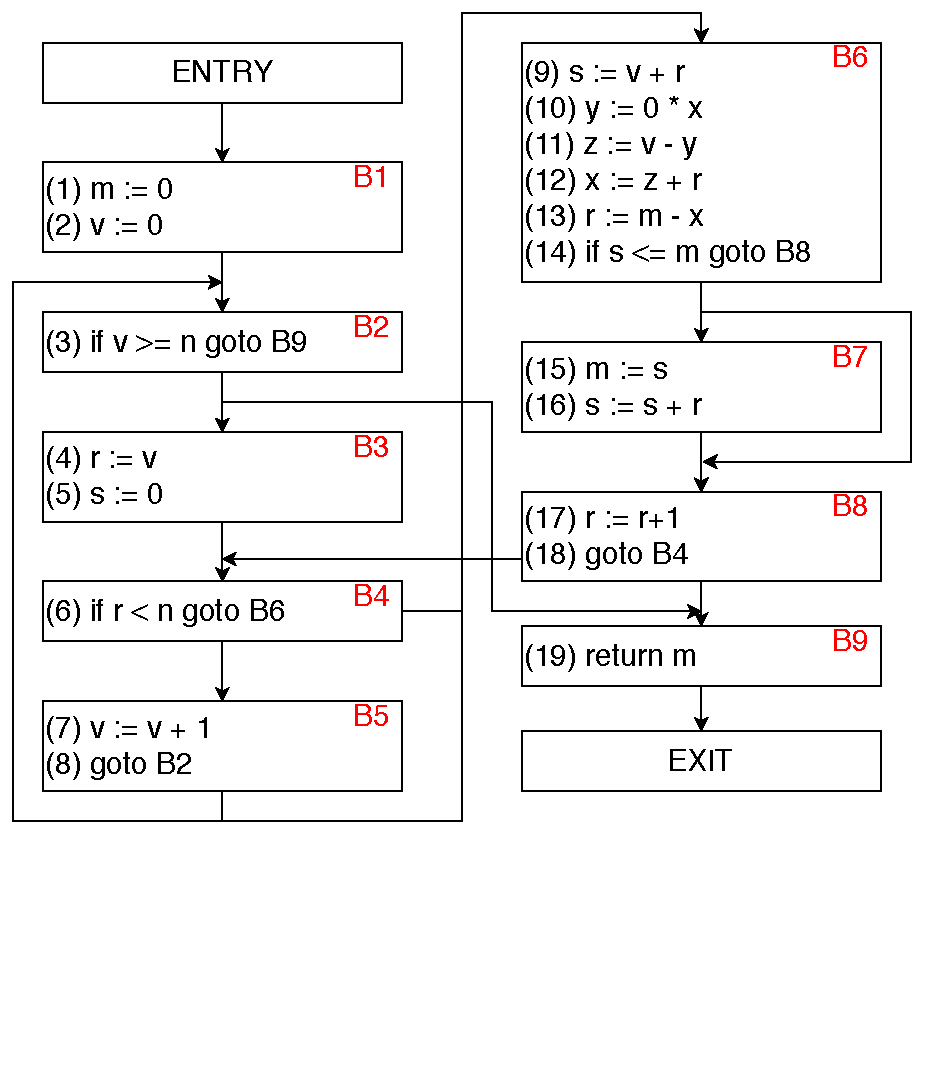
\includegraphics[width=0.7\linewidth]{fig/dag-2.pdf}
\end{figure}
\end{answer}

\end{document}